\documentclass[12pt, titlepage]{article}

\usepackage{fullpage}
\usepackage[round]{natbib}
\usepackage{multirow}
\usepackage{booktabs}
\usepackage{tabularx}
\usepackage{graphicx}
\usepackage{float}
\usepackage{hyperref}
\hypersetup{
    colorlinks,
    citecolor=blue,
    filecolor=black,
    linkcolor=red,
    urlcolor=blue
}

%% Comments

\usepackage{color}

\newif\ifcomments\commentstrue %displays comments
%\newif\ifcomments\commentsfalse %so that comments do not display

\ifcomments
\newcommand{\authornote}[3]{\textcolor{#1}{[#3 ---#2]}}
\newcommand{\todo}[1]{\textcolor{red}{[TODO: #1]}}
\else
\newcommand{\authornote}[3]{}
\newcommand{\todo}[1]{}
\fi

\newcommand{\wss}[1]{\authornote{blue}{SS}{#1}} 
\newcommand{\plt}[1]{\authornote{magenta}{TPLT}{#1}} %For explanation of the template
\newcommand{\an}[1]{\authornote{cyan}{Author}{#1}}

%% Common Parts

\newcommand{\progname}{Software Engineering} % PUT YOUR PROGRAM NAME HERE
\newcommand{\authname}{Team \#22, TeleHealth Insights
\\ Mitchell Weingust
\\ Parisha Nizam
\\ Promish Kandel
\\ Jasmine Sun-Hu} % AUTHOR NAMES                  

\usepackage{hyperref}
    \hypersetup{colorlinks=true, linkcolor=blue, citecolor=blue, filecolor=blue,
                urlcolor=blue, unicode=false}
    \urlstyle{same}
                                


\newcounter{acnum}
\newcommand{\actheacnum}{AC\theacnum}
\newcommand{\acref}[1]{AC\ref{#1}}

\newcounter{ucnum}
\newcommand{\uctheucnum}{UC\theucnum}
\newcommand{\uref}[1]{UC\ref{#1}}

\newcounter{mnum}
\newcommand{\mthemnum}{M\themnum}
\newcommand{\mref}[1]{M\ref{#1}}

\begin{document}

\title{Module Guide for \progname{}} 
\author{\authname}
\date{\today}

\maketitle

\pagenumbering{roman}

\section{Revision History}

\begin{tabularx}{\textwidth}{p{3cm}p{2cm}X}
\toprule {\bf Date} & {\bf Version} & {\bf Notes}\\
\midrule
Date 1 & 1.0 & Notes\\
Date 2 & 1.1 & Notes\\
\bottomrule
\end{tabularx}

\newpage

\section{Reference Material}

This section records information for easy reference.

\subsection{Abbreviations and Acronyms}

\renewcommand{\arraystretch}{1.2}
\begin{tabular}{l l} 
  \toprule		
  \textbf{symbol} & \textbf{description}\\
  \midrule 
  AC & Anticipated Change\\
  DAG & Directed Acyclic Graph \\
  M & Module \\
  MG & Module Guide \\
  OS & Operating System \\
  R & Requirement\\
  SC & Scientific Computing \\
  SRS & Software Requirements Specification\\
  \progname & Explanation of program name\\
  UC & Unlikely Change \\
  \wss{etc.} & \wss{...}\\
  \bottomrule
\end{tabular}\\

\newpage

\tableofcontents

\listoftables

\listoffigures

\newpage

\pagenumbering{arabic}

\section{Introduction}

Decomposing a system into modules is a commonly accepted approach to developing
software.  A module is a work assignment for a programmer or programming
team~\citep{ParnasEtAl1984}.  We advocate a decomposition
based on the principle of information hiding~\citep{Parnas1972a}.  This
principle supports design for change, because the ``secrets'' that each module
hides represent likely future changes.  Design for change is valuable in SC,
where modifications are frequent, especially during initial development as the
solution space is explored.  

Our design follows the rules layed out by \citet{ParnasEtAl1984}, as follows:
\begin{itemize}
\item System details that are likely to change independently should be the
  secrets of separate modules.
\item Each data structure is implemented in only one module.
\item Any other program that requires information stored in a module's data
  structures must obtain it by calling access programs belonging to that module.
\end{itemize}

After completing the first stage of the design, the Software Requirements
Specification (SRS), the Module Guide (MG) is developed~\citep{ParnasEtAl1984}. The MG
specifies the modular structure of the system and is intended to allow both
designers and maintainers to easily identify the parts of the software.  The
potential readers of this document are as follows:

\begin{itemize}
\item New project members: This document can be a guide for a new project member
  to easily understand the overall structure and quickly find the
  relevant modules they are searching for.
\item Maintainers: The hierarchical structure of the module guide improves the
  maintainers' understanding when they need to make changes to the system. It is
  important for a maintainer to update the relevant sections of the document
  after changes have been made.
\item Designers: Once the module guide has been written, it can be used to
  check for consistency, feasibility, and flexibility. Designers can verify the
  system in various ways, such as consistency among modules, feasibility of the
  decomposition, and flexibility of the design.
\end{itemize}

The rest of the document is organized as follows. Section
\ref{SecChange} lists the anticipated and unlikely changes of the software
requirements. Section \ref{SecMH} summarizes the module decomposition that
was constructed according to the likely changes. Section \ref{SecConnection}
specifies the connections between the software requirements and the
modules. Section \ref{SecMD} gives a detailed description of the
modules. Section \ref{SecTM} includes two traceability matrices. One checks
the completeness of the design against the requirements provided in the SRS. The
other shows the relation between anticipated changes and the modules. Section
\ref{SecUse} describes the use relation between modules.

\section{Anticipated and Unlikely Changes} \label{SecChange}

This section lists possible changes to the system. According to the likeliness
of the change, the possible changes are classified into two
categories. Anticipated changes are listed in Section \ref{SecAchange}, and
unlikely changes are listed in Section \ref{SecUchange}.

\subsection{Anticipated Changes} \label{SecAchange}

Anticipated changes are the source of the information that is to be hidden
inside the modules. Ideally, changing one of the anticipated changes will only
require changing the one module that hides the associated decision. The approach
adapted here is called design for
change.

\begin{description}
\item[\refstepcounter{acnum} \actheacnum \label{acHardware}:] The specific
  hardware on which the software is running.
\item[\refstepcounter{acnum} \actheacnum \label{acInput}:] The format of the
  initial input data.
\item ...
\end{description}

\wss{Anticipated changes relate to changes that would be made in requirements,
design or implementation choices.  They are not related to changes that are made
at run-time, like the values of parameters.}

\subsection{Unlikely Changes} \label{SecUchange}

The module design should be as general as possible. However, a general system is
more complex. Sometimes this complexity is not necessary. Fixing some design
decisions at the system architecture stage can simplify the software design. If
these decision should later need to be changed, then many parts of the design
will potentially need to be modified. Hence, it is not intended that these
decisions will be changed.

\begin{description}
\item[\refstepcounter{ucnum} \uctheucnum \label{ucIO}:] Input/Output devices
  (Input: File and/or Keyboard, Output: File, Memory, and/or Screen).
\item ...
\end{description}

\section{Module Hierarchy} \label{SecMH}

This section provides an overview of the module design. Modules are summarized
in a hierarchy decomposed by secrets in Table \ref{TblMH}. The modules listed
below, which are leaves in the hierarchy tree, are the modules that will
actually be implemented.

\begin{description}
\item [\refstepcounter{mnum} \mthemnum \label{mHH}:] Hardware-Hiding Module
\item ...
\end{description}


\begin{table}[h!]
\centering
\begin{tabular}{p{0.3\textwidth} p{0.6\textwidth}}
\toprule
\textbf{Level 1} & \textbf{Level 2}\\
\midrule

{Hardware-Hiding Module} & ~ \\
\midrule

\multirow{7}{0.3\textwidth}{Behaviour-Hiding Module} & ?\\
& ?\\
& ?\\
& ?\\
& ?\\
& ?\\
& ?\\ 
& ?\\
\midrule

\multirow{3}{0.3\textwidth}{Software Decision Module} & {?}\\
& ?\\
& ?\\
\bottomrule

\end{tabular}
\caption{Module Hierarchy}
\label{TblMH}
\end{table}

\section{Connection Between Requirements and Design} \label{SecConnection}

The design of the system is intended to satisfy the requirements developed in
the SRS. In this stage, the system is decomposed into modules. The connection
between requirements and modules is listed in Table~\ref{TblRT}.

\wss{The intention of this section is to document decisions that are made
  ``between'' the requirements and the design.  To satisfy some requirements,
  design decisions need to be made.  Rather than make these decisions implicit,
  they are explicitly recorded here.  For instance, if a program has security
  requirements, a specific design decision may be made to satisfy those
  requirements with a password.}

\section{Module Decomposition} \label{SecMD}

Modules are decomposed according to the principle of ``information hiding''
proposed by \citet{ParnasEtAl1984}. The \emph{Secrets} field in a module
decomposition is a brief statement of the design decision hidden by the
module. The \emph{Services} field specifies \emph{what} the module will do
without documenting \emph{how} to do it. For each module, a suggestion for the
implementing software is given under the \emph{Implemented By} title. If the
entry is \emph{OS}, this means that the module is provided by the operating
system or by standard programming language libraries.  \emph{\progname{}} means the
module will be implemented by the \progname{} software.

Only the leaf modules in the hierarchy have to be implemented. If a dash
(\emph{--}) is shown, this means that the module is not a leaf and will not have
to be implemented.

\subsection{Hardware Hiding Modules (\mref{mHH})}

\begin{description}
\item[Secrets:]The data structure and algorithm used to implement the virtual
  hardware.
\item[Services:]Serves as a virtual hardware used by the rest of the
  system. This module provides the interface between the hardware and the
  software. So, the system can use it to display outputs or to accept inputs.
\item[Implemented By:] OS
\end{description}

\subsection{Behaviour-Hiding Module}

\begin{description}
\item[Secrets:]The contents of the required behaviours.
\item[Services:]Includes programs that provide externally visible behaviour of
  the system as specified in the software requirements specification (SRS)
  documents. This module serves as a communication layer between the
  hardware-hiding module and the software decision module. The programs in this
  module will need to change if there are changes in the SRS.
\item[Implemented By:] --
\end{description}

\subsubsection{Media Processing Module (\mref{MediaProcessing})}
\begin{description}
\item[Secrets:] The design and implementation of how media (video and audio) is processed in the system.
\item[Services:] Provides high-level functionality for media processing by delegating tasks to its submodules: Video Processing Module and Audio Processing Module. Acts as an abstraction layer for handling media data.
\item[Implemented By:] Media-processing-service
\item[Type of Module:]  Abstract Object
\end{description}

\subsubsection{Video Processing Module (\mref{VideoProcessing})}
\begin{description}
\item[Secrets:] The methods and algorithms used to process video data, including frame extraction, format handling, and metadata processing.
\item[Services:] Handles all video-related data processing tasks, such as analyzing video frames, ensuring quality, and extracting relevant details. This module communicates with the Media Processing Module.
\item[Implemented By:] Media-processing-service
\item[Type of Module:]  Abstract Object
\end{description}

\subsubsection{Audio Processing Module (\mref{AudioProcessing})}
\begin{description}
\item[Secrets:] The methods and algorithms used to process audio data, such as format conversions, noise filtering, and speech analysis.
\item[Services:] Handles all audio-related data processing tasks, including speech detection, sound quality analysis, and extracting key audio features. This module communicates with the Media Processing Module.
\item[Implemented By:] Media-processing-service
\item[Type of Module:] Abstract Object
\end{description}

\subsubsection{Logging Module (\mref{mLogging})}
\begin{description}
\item[Secrets:] The design and implementation of log storage and retrieval mechanisms, as well as the structure of the logs (e.g., event logs, error logs, debug logs).
\item[Services:] Tracks system activity and errors through event logging. Supports audit logging for user actions and system changes.
Provides interfaces to query and clear logs for maintenance.
\item[Implemented By:] logging-monitoring-service
\item[Type of Module:] List of Records
\end{description}

\subsection{Software Decision Module}

\section{Traceability Matrix} \label{SecTM}

This section shows two traceability matrices: between the modules and the
requirements and between the modules and the anticipated changes.

% the table should use mref, the requirements should be named, use something
% like fref
\begin{table}[H]
\centering
\begin{tabular}{p{0.2\textwidth} p{0.6\textwidth}}
\toprule
\textbf{Req.} & \textbf{Modules}\\
\midrule
FR-A1 & M1, M2, M3, M5, M8 \\
FR-A2 &  M2, M3,  M5, M8 \\
FR-A3 &  M1,M3, M5, M8 \\
FR-A4 & M5, M8\\
FR-A5 & M5, M8 \\
FR-SS1 & M2, M3 \\
FR-SS2 & M2, M3\\
FR-SS3 & M2, M3\\
FR-SS4 & M2, M3 \\
FR-SS5 & M2, M3, M9\\
FR-AI1 & M2, M3, M7, M9, M12, M13, M14, M15, M16 \\
FR-AI2 & M2, M3, M4, M7, M9, M12, M13, M14, M15, M16 \\
FR-AI3 & M2, M3, M4, M7, M9, M12, M13, M14, M15, M16 \\
FR-AI4 & M2, M3, M4, M7, M9, M12, M13, M14, M15, M16 \\
FR-AI5 & M2, M3, M4, M7, M9, M12, M13, M14, M15, M16 \\
FR-AI6 & M2, M3, M4, M6, M7, M9 M12, M13, M14, M15, M16 \\
FR-AI7 & M2, M3, M4, M7, M9 M12, M13, M14, M15, M16, M17 \\
FR-DSC1 & M4, M6, M8, \\
FR-DSC2 & M4, M6, M7, M10, M12, M13 \\
FR-DSC3 & M4, M5\\
FR-DSC4 & M4, M5 \\
FR-DSC5 & M4, M8, M10, M11 \\
FR-VADA1 & M4, M7, M12, M13 \\
FR-VADA2 & M4, M7,M8 M12, M13 \\
FR-VADA3 & M4, M7, M8, M12, M13 \\
FR-DPD1 & M4, M6, M8, M10, M11 \\
FR-DPD2 & M4, M6, M8, M10, M11\\
FR-DPD3 & M1, M4, M6, M8, M10, M11\\
FR-DPD4 & M1, M4, M6, M8, M10, M11\\


\bottomrule
\end{tabular}
\caption{Trace Between Requirements and Modules}
\label{TblRT}
\end{table}

\begin{table}[H]
\centering
\begin{tabular}{p{0.2\textwidth} p{0.6\textwidth}}
\toprule
\textbf{AC} & \textbf{Modules}\\
\midrule
AC1 & M9, M17 \\
AC2 & M9, M16, M17 \\
\end{tabular}
\caption{Trace Between Anticipated Changes and Modules}
\label{TblACT}
\end{table}

\section{Use Hierarchy Between Modules} \label{SecUse}

In this section, the uses hierarchy between modules is
provided. \citet{Parnas1978} said of two programs A and B that A {\em uses} B if
correct execution of B may be necessary for A to complete the task described in
its specification. That is, A {\em uses} B if there exist situations in which
the correct functioning of A depends upon the availability of a correct
implementation of B.  Figure \ref{FigUH} illustrates the use relation between
the modules. It can be seen that the graph is a directed acyclic graph
(DAG). Each level of the hierarchy offers a testable and usable subset of the
system, and modules in the higher level of the hierarchy are essentially simpler
because they use modules from the lower levels.

\wss{The uses relation is not a data flow diagram.  In the code there will often
be an import statement in module A when it directly uses module B.  Module B
provides the services that module A needs.  The code for module A needs to be
able to see these services (hence the import statement).  Since the uses
relation is transitive, there is a use relation without an import, but the
arrows in the diagram typically correspond to the presence of import statement.}

\wss{If module A uses module B, the arrow is directed from A to B.}

\begin{figure}[H]
\centering
%\includegraphics[width=0.7\textwidth]{UsesHierarchy.png}
\caption{Use hierarchy among modules}
\label{FigUH}
\end{figure}

%\section*{References}

\section{User Interfaces}

\wss{Design of user interface for software and hardware.  Attach an appendix if
needed. Drawings, Sketches, Figma}

\hspace{1.5em}The interfaces below depicts the interface allowing a user who enters the application to either login to the platform if they have an existing account, or create a new account for new users.
\begin{figure}[H]
  \centering
  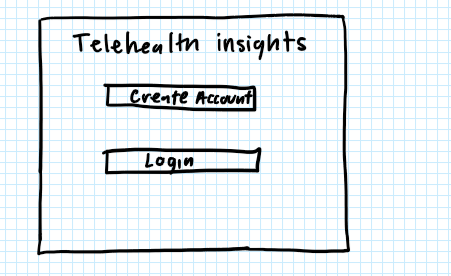
\includegraphics[scale=0.9]{images/createORlogin.png}
  \caption{Login or Create an Account}
\end{figure}

\hspace{1.5em}The interfaces below depicts the flow of selecting which account type to create. If a parent account is chosen, they are able to create a username and password and enter client number to complete the account creation. A clinician account information with be created and provided to the clinician by the admin.
\begin{figure}[H]
  \centering
  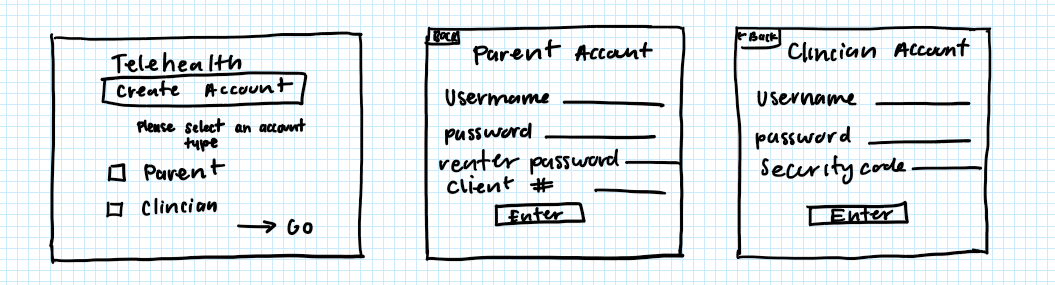
\includegraphics[scale=0.9]{images/create account.png}
  \caption{Create an Account}
\end{figure}

\hspace{1.5em}The interface below depicts the login page overview, where a user can login to the application if they already have an existing account.
\begin{figure}[H]
  \centering
  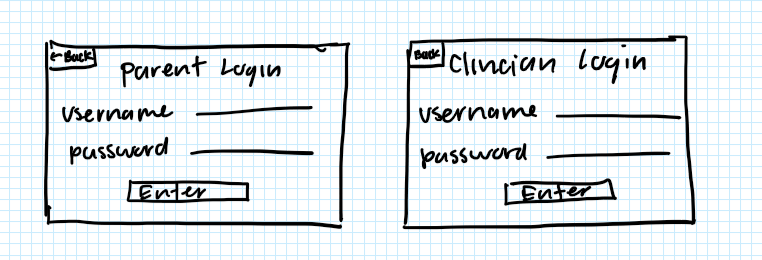
\includegraphics[scale=0.9]{images/loginaccount.png}
  \caption{Login in to account}
\end{figure}

\hspace{1.5em}The interface below depicts the home page for the parent to enter the assesement platform. The home page provides options to learn how to use the assessment platform or start the assessment. 
\begin{figure}[H]
  \centering
  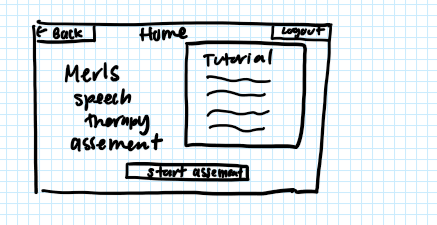
\includegraphics[scale=0.9]{images/homepage.png}
  \caption{Parent HomePage}
\end{figure}

\hspace{1.5em}The below finite state machine depicts how the parent can interface with the homepage, as well as which interactions lead to changes in states in the system for logging in/out with authentication.
\begin{figure}[H]
  \centering
  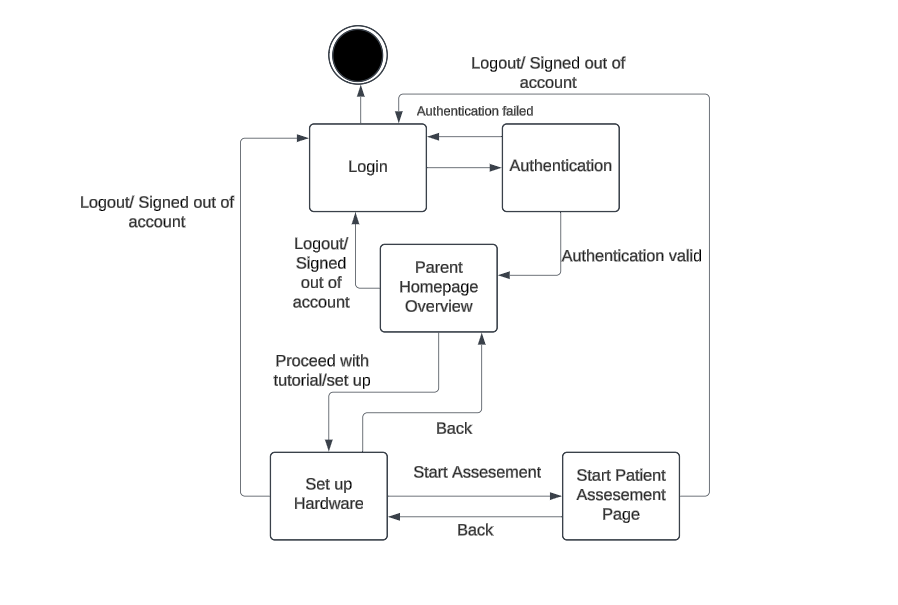
\includegraphics[scale=0.6]{images/FSM Homepage.png}
  \caption{FSM - Parent Homepage}
\end{figure}



\section{Design of Communication Protocols}

\wss{If appropriate}

\section{Timeline}

\wss{Schedule of tasks and who is responsible}

\wss{You can point to GitHub if this information is included there}

\bibliographystyle {plainnat}
\bibliography{../../../refs/References}

\newpage{}

\end{document}